\documentclass[12pt,a4paper,twoside]{report}
\usepackage[utf8]{inputenc}
\usepackage[english]{babel}
\usepackage{ragged2e}
\usepackage{parskip}
\usepackage{xcolor}
\usepackage{graphicx}
\usepackage{geometry}
\usepackage{titlesec}
\usepackage{textcomp}
\usepackage{enumitem}
\usepackage{newunicodechar}
\usepackage{booktabs}
\usepackage{tabularx}
\usepackage{float}
\usepackage{longtable}
\usepackage{xltabular}
\usepackage{ragged2e}
\usepackage{caption}
\usepackage{url}
\usepackage[hidelinks]{hyperref}
\usepackage[table]{xcolor}
\usepackage[helvetica]{quotchap}
\usepackage[font=normalsize,labelfont={bf}]{caption}
\usepackage[backend=biber, style=ieee, giveninits=true]{biblatex}
\usepackage{appendix}

% Margins
\geometry{left=2.5cm, right=2.5cm, top=2.5cm, bottom=2.5cm}

% Add blankpages
\newcommand{\blankpage}{
\newpage
\thispagestyle{empty}
\mbox{}
\newpage
}

% Add references
\addbibresource{refs.bib}
\setlength\bibitemsep{\baselineskip}
\DeclareFieldFormat{urldate}{}

% Font color
\definecolor{indigo}{HTML}{1F497D}

% Font for tables
\definecolor{lightgray}{HTML}{EEEEEE}


% Change chapter format
% \titleformat{\chapter}
% {\normalfont\LARGE\bfseries}{\thechapter.}{1em}{}
\renewcommand{\sectfont}{\bfseries}
\renewcommand{\chapterheadstartvskip}



% Trademark symbol as a superscript
\newcommand{\regsup}{\textsuperscript{\textregistered}}

% Tiny textbullet
\newunicodechar{•}{\textbullet}

\hypersetup{
    colorlinks=true,
    linkcolor=black, 
    citecolor=black, 
    urlcolor=blue    
}

\captionsetup{font=footnotesize}

% Parts of the document
\begin{document}

\justifying{}
    % Stop page numbering for preliminary sections
    \pagenumbering{gobble}
    \begin{titlepage}

    \begin{flushright}
        
\includegraphics[width=0.095\textwidth]{img/dna.jpg}
    \end{flushright}

    \centering
    \vspace{0.8cm}

    \Huge
    \textbf{Exploring Structural Variation in Tumor Evolution
    through Nanopore Sequencing}

    \vspace{0.8cm}

    \large
    \textbf{Student: Francisco José Villena González}

    \vspace{0.8cm}

    \large
    MASTER'S DEGREE IN BIOINFORMATICS AND DATA SCIENCE \\
    FOR PRECISION PERSONALIZED MEDICINE AND HEALTH

    \vspace{0.25cm}
    \large
    2023--2024

    \vspace{0.9cm}

    
\includegraphics[width=0.5\textwidth]{img/logo-ministerio.png}
    
    \vspace{0cm}
    
    
\includegraphics[width=0.5\textwidth]{img/logo_ISCIII.jpg}

    \vspace{0.8cm}

    \begin{flushleft}
        \large
        \textcolor{indigo}{Bioinformatics Unit of the Spanish National 
        Cancer Research Centre}
        
        Master's Thesis Supervisor: \textcolor{indigo}{Tomás Di Domenico} 
        
        Submission Date: \textcolor{indigo}{15 de enero de 2025}
    \end{flushleft}

    \vfill

    \begin{minipage}[t]{0.20\textwidth}
        
\includegraphics[width=\textwidth]{img/logo-ENS.jpg}
    \end{minipage}
    \hfill
    \begin{minipage}[t]{0.20\textwidth}
        
\includegraphics[width=\textwidth]{img/sebiot_logo.png}
    \end{minipage}
    \hfill
    \begin{minipage}[t]{0.35\textwidth}
        
\includegraphics[width=\textwidth]{img/biysc_bsc_logo.png}
    \end{minipage}
    \hfill
    \begin{minipage}[t]{0.17\textwidth}
        
\includegraphics[width=\textwidth]{img/cnio_logo.png}
    \end{minipage}

\end{titlepage}

    \blankpage{}

    \begin{center}
    \Large\bfseries Exploring Structural Variation in Tumor Evolution through 
    Nanopore Sequencing

\end{center} 

\vspace{0.5cm}
    \noindent\textbf{\large Abstract:}

    Structural variants (SVs) are genomic alterations encompassing deletions, 
    insertions, and segment rearrangements, ranging from kilobases to entire 
    chromosomes. Despite their significance as biomarkers in oncological 
    diseases, these variants have remained relatively unexplored compared to 
    single nucleotide variants, largely due to the inherent limitations of 
    short-read sequencing technologies that have dominated large-scale genome 
    sequencing projects. This scenario has undergone a transformative change 
    with the advent of long-read sequencing technologies, which have enabled 
    the achievement of the first truly complete human telomere-to-telomere 
    reference genome, successfully filling gaps that short reads could not 
    resolve. This project focuses on conducting a comprehensive performance 
    evaluation of long-read-based structural variant callers, specifically in 
    the context of tumor evolution analysis. To address the limited availability
    of appropriate datasets, we have developed specialized workflows leveraging 
    high-performance computing resources for generating synthetic data with 
    custom SVs, thus facilitating robust benchmarking of various structural 
    variant detection methods. This computational approach enables systematic 
    evaluation of SV detection algorithms under controlled conditions, 
    providing valuable insights into their performance and reliability.


\vspace{0.5cm}
    \noindent\textbf{\large Key words:} 
    
    Structural Variants, Cancer Genomics, Oxford Nanopore Sequencing, Long-Read 
    Sequencing, High Performance Computing, Synthetic Data Generation, Variant 
    Calling, Bioinformatics.


    \blankpage{}

    \vspace{0.5cm}
    \noindent\textbf{\large Acknowledgements:}

    Quiero empezar dando las gracias a Tomás, por haber sido y querer 
    seguir siendo el mentor de este \textit{bio} con interés por acercarse
    mucho más a lo \textit{info}. También por romper mi maldición con los nanoporos,
    haciendo que este máster sobrepase todas mis expectativas.

    Gracias a Fátima por incluirme entre sus filas en la Unidad de Bioinformática,
    y a todo el equipo, gracias a vosotros (y a los mixtos con huevo de la cafetería) 
    la opción de teletrabajar se hace mucho menos atractiva.

    Gracias a la Fundación Instituto Roche por la ayuda económica para cursar
    este máster, lo de que el dinero no da la felicidad es una mentira 
    refutada por los que podemos seguir haciendo aquello que nos apasiona
    gracias a las becas.
    
    Por último, a los culpables de que estos agradecimientos hayan sido en 
    español, Nieves y Paco, mis padres. Gracias a sus esfuerzos he podido vivir 
    la vida con el privilegio de también poder estudiarla.



    \blankpage{}

    % Index
    \tableofcontents
    \blankpage{}

    \listoffigures
    \blankpage{}

    \listoftables
    \blankpage{}

    % Start page numbering
    \clearpage
    \pagenumbering{arabic}
    \setcounter{page}{1}
    % \AddLabels
    \chapter{Introduction}

\section{Sequencing Technologies in Cancer Research}

% Las secuencias genómicas ejercen elevada influencia sobre la biología de los 
% organismos y permiten inferir su historia evolutiva. 


% SECUENCIAS GENOMICAS Y MEDICINA DE PRECISIÓN

Genomic sequences significantly influence organismal biology and provide 
insights into evolutionary history. The application of this genomic knowledge 
to human health has given rise to precision medicine, a discipline that 
leverages genetic and molecular markers to personalize medical treatments 
according to individual patient characteristics \cite{collins_new_2015}. 
Advances in sequencing platforms and bioinformatics tools have enabled the 
identification of genetic variations that predispose individuals to specific 
diseases, facilitating the design of targeted therapies that enhance efficacy 
while reducing side effects \cite{carrasco-ramiro_human_2017}.

In oncology, genomic analyses have revolutionized our understanding and 
therapeutic approach to cancer \cite{johannessen_progress_2017}. According to 
the National Cancer Institute (NCI), cancer encompasses more than 100 distinct 
types, arising when normal cells undergo genetic and/or epigenetic alterations 
leading to uncontrolled proliferation and compromised organismal homeostasis
\cite{nci_what_2007}. Cancer development represents a complex process resulting 
from interactions between individual genotype and various environmental 
factors, driving clonal evolution where distinct malignant cell subpopulations 
compete for resources and space \cite{turajlic_resolving_2019}. Tumor DNA 
sequencing enables identification of patient-specific driver mutations, 
facilitating more effective targeted therapy selection and implementation 
\cite{sicklick_molecular_2019}.

% Las secuencias genómicas ejercen una elevada influencia sobre la biología de los 
% organismos y permiten inferir su historia evolutiva. La aplicación de esta 
% información en el ámbito de la salud humana ha dado lugar a lo que se conoce 
% como medicina de precisión. Esta disciplina, mediante el uso de marcadores 
% genéticos y moleculares, permite personalizar los tratamientos médicos, 
% adaptándolos a las características individuales de cada paciente. Gracias a los 
% avances en las plataformas de secuenciación y de herramientas bioinformáticas,
% es posible identificar variaciones genéticas que predisponen a ciertas 
% enfermedades y diseñar terapias específicas que mejoran la eficacia y reducen 
% los efectos secundarios.

% En el contexto del cáncer, los análisis genómicos han revolucionado nuestra 
% comprensión y abordaje terapéutico de la enfermedad. El cáncer, que engloba 
% más de 100 tipos diferentes según el Instituto Nacional del Cáncer (NCI), surge 
% cuando las células normales experimentan alteraciones genéticas y/o epigenéticas 
% que las llevan a proliferar de forma descontrolada, comprometiendo la 
% homeostasis del organismo. Su desarrollo es un proceso complejo que resulta de 
% la interacción entre el genotipo del individuo y diversos factores ambientales, 
% dando lugar a una evolución clonal donde distintas subpoblaciones de células 
% malignas compiten por recursos y espacio. La secuenciación del ADN tumoral 
% permite identificar las mutaciones específicas que impulsan el crecimiento 
% canceroso en cada paciente, facilitando la selección de terapias dirigidas más 
% efectivas.

DNA sequencing methods have evolved significantly over the years, with current 
technologies falling into three main categories:

\begin{itemize}[label=\tiny\raise.5ex\hbox{•}, leftmargin=\parindent]
    
    \item \textbf{Chain-termination method}: Also known as Sanger sequencing 
    after its primary developer, this technique relies on controlled DNA synthesis 
    termination, generating fragments of varying lengths that reveal the original 
    sequence when size-separated. While largely superseded for genomic projects 
    due to its low throughput, it remains valuable in research for verifying 
    short reads such as PCR products from individual genes 
    \cite{moorcraft_understanding_2015}.

    \item \textbf{Short-read sequencing}: Technologies that perform massive 
    parallel sequencing of clonally amplified DNA fragments (250-600 bp), 
    delivering high sequencing depths with $>$99.9\% accuracy
    \cite{logsdon_long-read_2020}. Illumina dominates this category globally, 
    though recent years have seen competition from MGI Tech, which promises 
    faster, more cost-effective high-quality sequencing
    \cite{jeon_comparison_2021}.

    \item \textbf{Long-read sequencing}: This approach also employs parallel 
    sequencing strategies but generates individual reads spanning tens to 
    thousands of kilobases. Currently, two main methods dominate this field: 
    Single Molecule Real-Time (SMRT) sequencing, commercialized by PacBio, and 
    nanopore sequencing, pioneered by Oxford Nanopore Technologies (ONT) 
    \cite{logsdon_long-read_2020} with the recent appearence of MGI Tech as
    possible alternative \cite{zhang_single-molecule_2024}.

\end{itemize}

\subsection{Limitations of Short-read Genome Assembly}

Cancer is largely driven by somatic changes in the genome, which can range from 
small nucleotide substitutions to chromosome-scale rearrangements. In this context, 
sequencing technologies play a crucial role, with predominant short-read sequencing 
having revolutionized our understanding of point mutations. However, this 
approach proves insufficient for resolving most large genomic alterations and 
generating gap-free assemblies. This limitation stems from the inherent 
inability of short reads (typically 150-300 base pairs) to span complex genomic 
regions, particularly those containing repetitive elements or large structural 
variations \cite{ho_structural_2020}. Furthermore, the fragmented nature of short 
reads complicates the accurate reconstruction of complex genomic architectures, 
often leading to ambiguous or incomplete assemblies 
(\textbf{Figure~\ref{fig:assembly_gaps}}).

\begin{figure}[H]
    \centering
    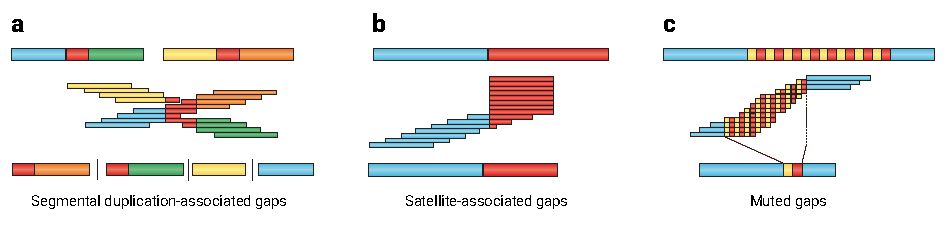
\includegraphics[width=\textwidth]{img/assembly_gaps.pdf}
    \caption[Limitations of short-read genome assembly]{Limitations of short-read 
    genome assembly. The upper bar of each figure shows regions to be resolved, 
    with repetitive sequences highlighted in red. The middle displays 
    short-read alignments, while the bottom bar shows the inferred sequence. 
    (\textbf{a}) Large segmental duplications of high sequence identity (orange 
    and green) create ambiguous read overlaps, resulting in multiple gaps flanking 
    segmental duplications. (\textbf{b}) Satellite-associated gaps represent 
    a special case causing read 'pileups' due to higher-order tandem arrays of 
    repetitive sequences, primarily occurring in centromeric, acrocentric, and 
    telomeric genomic regions. (\textbf{c}) Muted gaps occur when the assembled 
    sequence appears shorter than the actual genome, typically in repetitive 
    regions that are difficult to amplify or are toxic to bacterial cloning, 
    such as simple tandem repeats. Adapted from \cite{chaisson_genetic_2015}.}
    % \caption[Algunas limitaciones en ensamblajes genómicos con lecturas cortas]{
    % Algunas limitaciones en ensamblajes genómicos con lecturas cortas. Encima De
    % cada figura están representadas las regiones a ser resueltas y las zonas
    % coloreadas de rojo son secuencias repetitivas. En medio de cada figura se 
    % muestran los alineamientos de lecturas cortas, y abajo del todo se encuentra
    % la secuencia que se ha sido inferida. (a) Large segmental duplications of 
    % high sequence identity, in orange and green, make read overlaps ambiguous, leading
    % to multiple gaps flanking segmental duplications. The effect becomes exacerbated 
    % if the duplications are structurally polymorphic in a diploid genome. (b)
    % Satellite-associated gaps are a special case leading to read ‘pileups’ due 
    % to higher-order tandem arrays of repetitive sequence, These occur primarily in centromeric,
    % acrocentric and telomeric areas of genomes. (c) Muted gaps arise when the 
    % assembly is contracted relative to the true genome when overlaps are consistent 
    % with a smaller representation of the genome. These are often associated with
    % repetitive sequences that cannot be easily amplified and/or are incompatible 
    % with cloning and propagation (that is, when they are toxic to Escherichia coli), 
    % such as simple tandem repeats.}
    \label{fig:assembly_gaps}
\end{figure}

\subsection{Long-read Contributions to Genome Assembly}

Long-read sequencing technologies emerged a decade ago, marking a turning point 
in sequence assembly by addressing short-read limitations. Initially, these 
technologies had much higher error rates (~10\%) compared to short reads ($<$ 1\%)
\cite{espinosa_advancements_2024}. While this enabled routine bacterial genome 
assembly, it limited their application in human genomics, particularly for point 
mutation detection \cite{loman_complete_2015}. However, continuous improvements 
in long-read sequencing platforms have progressively reduced these error rates, 
ultimately enabling the generation of the first gap-free human reference genome, 
known as telomere-to-telomere (T2T) assembly \cite{nurk_complete_2022}. 
This achievement resolved previously inaccessible genomic regions that remained 
incomplete in the Genome Reference Consortium's human reference version 38 
(GRCh38), highlighted in red in \textbf{Figure~\ref{fig:T2T_ref}}.

% The advent of Las tecnologías de secuenciación de lecturas largas hace una
% década con el potencial de superar las limitaciones de las lecturas cortas,
% and marked a turning point in sequence assembly. Sin embargo, esas long reads 
% tenían higher error rate (~10\%) than short reads ($<$ 1\%), it was practical to 
% routinely assemble complete bacterial genome, pero desincentivaba su uso
% en genómica humana debido a no ser útiles en el análisis de mutaciones puntuales.
% No obstante, las continuas mejoras de las plataformas de secuenciación basadas
% en long-reads han ido reduciendo estos error rates, hasta el punto de permitir 
% generar el primer genoma humano de referencia sin gaps, también denominado 
% telómero a telómero (T2T), adressing genomic regions remained unresolved in the
% la versión 38 de la referencia humana lanzada por el Genome Reference Consortium
% (GRCh38).

\begin{figure}[H]
    \centering
    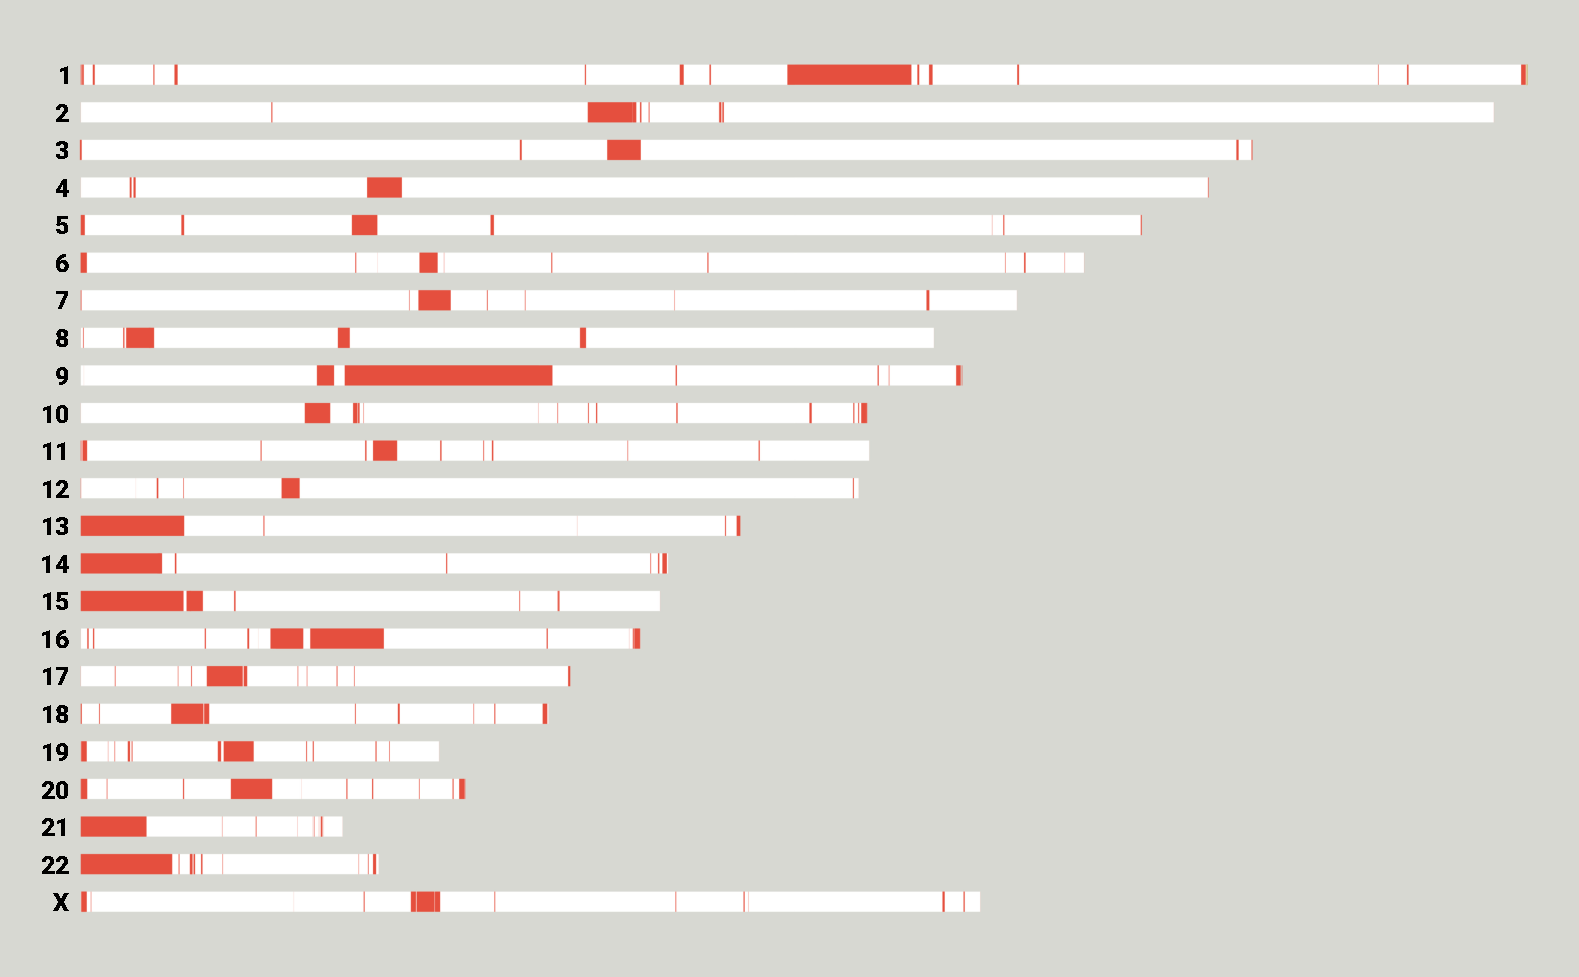
\includegraphics[width=\textwidth]{img/T2T_ref.pdf}
    \caption[Gaps resolved by T2T assembly]{Gaps resolved by T2T assembly. Each 
    bar represents a linear visualization of a chromosome, with chromosome 
    numbers indicated on the left. Red segments denote previously missing 
    sequences resolved by the T2T Consortium in 2022. The Y chromosome is not 
    included, as its complex architecture, particularly its large, tandemly 
    arrayed and inverted repeats (IRs), required additional analysis and was 
    published separately in 2023 \cite{rhie_complete_2023}. Adapted from 
    \cite{zahn_filling_2022}.}
    % \caption[Gaps resolved by T2T assembly]{Gaps resolved by T2T assembly. 
    % Each bar is a linear visualization of a chromosome, with the chromosome 
    % number shown at left. Red segments denote previously missing sequences that 
    % the T2T Consortium resolved in 2022. No se incluye el cromosoma Y, debido
    % a que fue publicado posteriormente en 2023 debido a su compleja arquitectura,
    % specifically the presence of large, tandemly arrayed and inverted repeats (IRs).}
    \label{fig:T2T_ref}
\end{figure}

Beyond sequencing methodology, significant differences exist between long-read 
platforms. Although PacBio pioneered the field in 2011 with high-throughput 
sequencing systems, their platforms have consistently required investments in 
the hundreds of thousands of dollars. In contrast, ONT's 2014 launch of MinION 
introduced a low-throughput but highly portable device requiring only a few 
thousand dollars investment. Subsequently, ONT expanded into high-throughput 
PromethION devices, notably the ``P2 solo'' model, which enables Whole Genome 
Sequencing (WGS) with a computer connection at under \$20,000. This 
cost-effective solution makes long-read sequencing accessible to virtually any 
molecular biology laboratory \cite{espinosa_advancements_2024,noauthor_vega_nodate,oxford_nanopore_technologies_nanopore_nodate}.

ONT sequencing technology operates by measuring ionic current changes as 
single-stranded DNA molecules thread through nanoscale pores embedded in a 
membrane. Each nucleotide's unique shape creates distinctive current 
perturbations as it passes through the pore, enabling sequence determination 
and even modified bases detection. These nanopores are arranged in arrays across 
a flow cell, ONT's core consumable component, which contains thousands of 
individual sensing channels. Each flow cell integrates microfluidics for sample 
delivery, electronics for current measurement, and an application-specific 
integrated circuit (ASCI) that enables real-time data collection from multiple 
nanopores simultaneously (\textbf{Figure~\ref{fig:ont_seq}}). 

\begin{figure}[H]
    \centering
    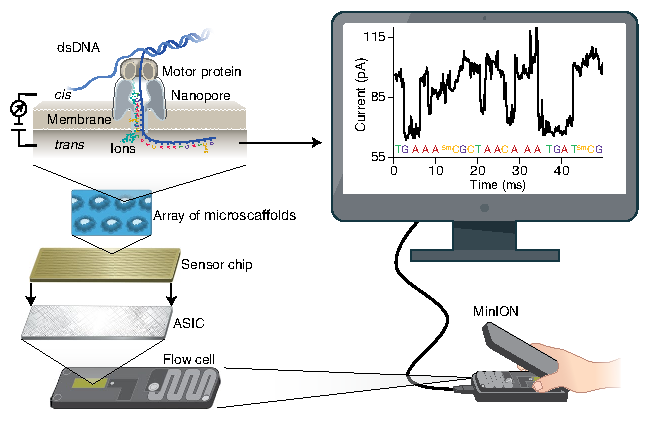
\includegraphics[width=0.8\textwidth]{img/ont_seq.pdf}
    \caption[Principle of nanopore sequencing]{Schematic representation of 
    nanopore sequencing using MinION technology. The diagram shows the key 
    components: nanopore embedded in a membrane, array of microscaffolds, 
    sensor chip, ASIC, and flow cell. The ionic current measurement graph 
    displays the characteristic signal patterns produced as DNA strands pass 
    through the nanopore. Adapted from \cite{wang_nanopore_2021}.}
    \label{fig:ont_seq}
\end{figure}

Recent improvements in both the nanopore architecture of flow cells 
(transitioning from the R9 pore protein, with a 9 Å constriction, to the R10 
variant featuring a longer barrel and 10 Å constriction) and basecalling 
algorithms have significantly enhanced sequence accuracy 
(\textbf{Figure~\ref{fig:ONT_updates}}), making long-read sequencing a viable 
approach for the systematic analysis of cancer-associated variation
\cite{kolmogorov_scalable_2023,sakamoto_phasing_2022,schaal_migrating_2022}.

\begin{figure}[H]
    \centering
    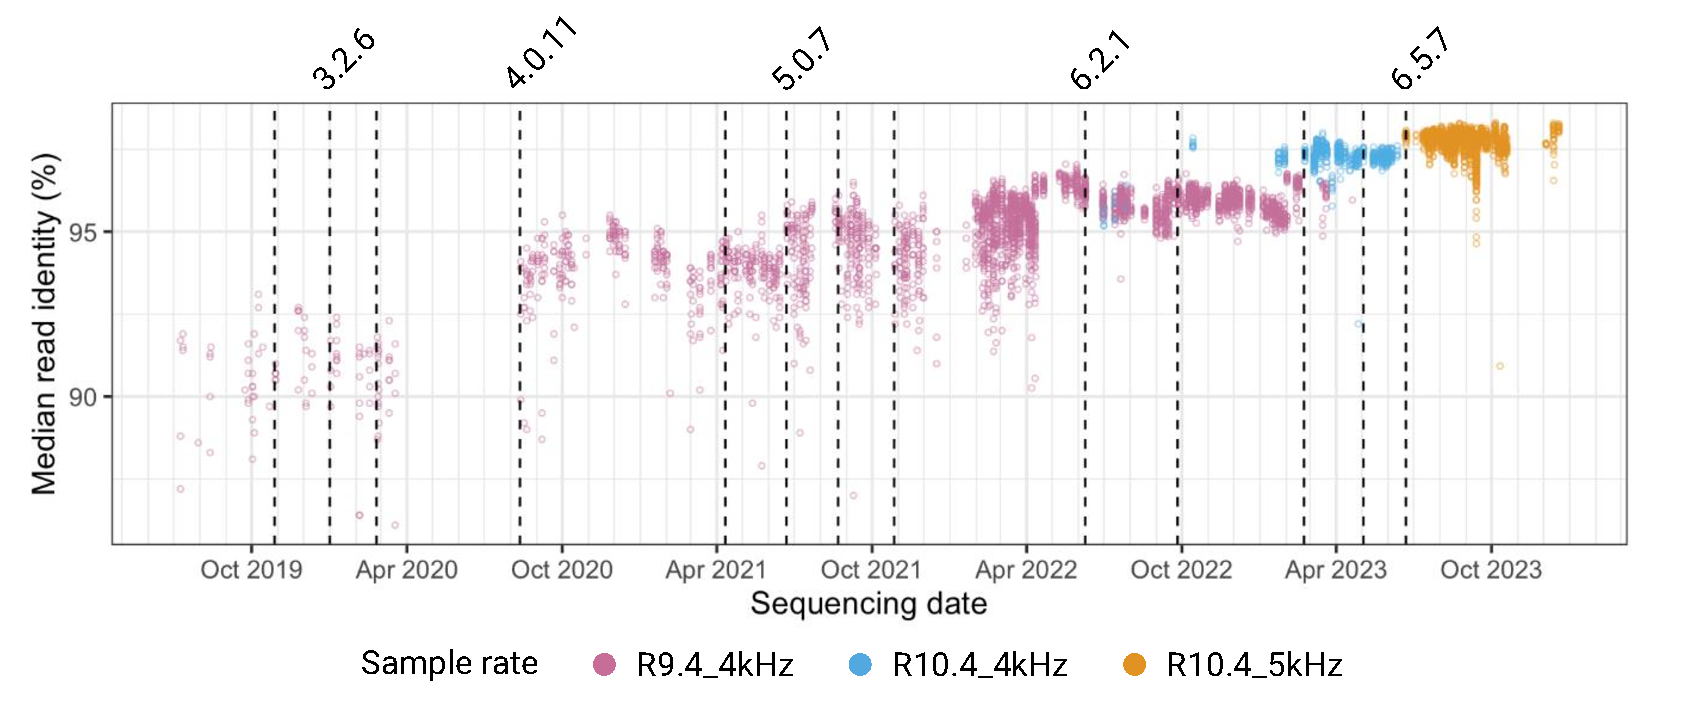
\includegraphics[width=\textwidth]{img/ONT_updates.pdf}
    \caption[Evolution of ONT basecalling accuracy]{Temporal evolution of median 
    read accuracy using Oxford Nanopore's Guppy basecaller versions shown 
    above. Each data point represents a human WGS experiment at 20-30x coverage 
    depth. Colors indicate the flowcell version and sampling rate: R9.4\_4kHz 
    (pink), R10.4\_4kHz (blue), and R10.4\_5kHz (orange), where sampling rate 
    (kHz) represents the number of electrical measurements per second during 
    sequencing (1 kHz = 1,000 measurements per second). Data from Genomics 
    England's R\&D Department, presented in ONT's Webinar ``Unlocking 
    comprehensive genome for large-scale projects'', courtesy of Adam Giess and 
    Melanie Tanguy \cite{oxford_nanopore_technologies_unlocking_2024}.}
    \label{fig:ONT_updates}
\end{figure}

The assembly of the first T2T genome required inputs from multiple platforms: 
PacBio for long and accurate HiFi data (15--25 kb at 99.5\% accuracy), 
ONT for ultra-long (UL) data ($>$100 kb at 95\% accuracy), and Illumina' 
short-reads (0.15 kb at 99.99\% accuracy) \cite{li_genome_2024}. While this 
combination of data types proved effective, it complicated data generation and 
limited accessibility. Currently, ONT provides all three sequencing modes on a 
single instrument using R10.4 PromethION flow cells, specific assembly chemistry 
kits, and associated bioinformatic workflows, resulting in automated assemblies 
with base accuracy exceeding 99.999\% and near-perfect continuity
\cite{koren_gapless_2024}. This is particularly promising as it opens up the 
possibility of generating personalized human genomes using PromethION sequencers 
for precision medicine research purposes.

\subsection{Structural Variation in Cancer}

Structural variants (SVs) are genomic alterations ranging from 50 pb to 
whole-chromosome events, including deletions, insertions, and segment 
rearrangements. The significance of SVs as a hallmark of cancer is becoming 
increasingly evident. A recent analysis of 2,658 tumor genomes revealed that 
approximately 50\% of driver mutations overlap with SVs, highlighting their 
crucial role in cancer development \cite{li_patterns_2020,menghi_tandem_2018}. 
Despite their importance as biomarkers in oncological diseases, our 
understanding of SVs remains limited compared to single nucleotide variants 
(SNVs). This knowledge gap stems primarily from the technical limitations of 
short-read sequencing, which has dominated large-scale genome sequencing 
projects. Using short reads, SV detection mainly relies on copy number variation 
(CNV) estimates, an indirect measure that fails to capture copy-number neutral 
events, inversions, and balanced translocations. Consequently, many 
cancer-driving SVs escape discovery using traditional short-read sequencing 
\cite{cameron_comprehensive_2019,abel_mapping_2020}.

The emergence of long-read sequencing technologies has marked a turning point in 
SV analysis, enabling improved variation detection in cancer genomes. A pioneering 
study using medulloblastoma cells, a primary childhood brain tumor, analyzed samples 
at diagnosis and post-treatment using long-read sequencing. This approach led to 
the identification of a novel mutational pattern called templated insertion (TI) 
thread, characterized by short ($<$1 kb) insertions that self-concatenate into highly 
amplified structures up to 50 kbp in size. This pattern was subsequently confirmed 
in other cancer types, showing particular prevalence in liposarcomas and frequent 
co-occurrence with chromothripsis, a catastropic mutational event where 
chromosomes shatter and reassemble chaotically \cite{rausch_long-read_2023}.

Long-read sequencing has also enabled the characterization of novel mutation 
mechanisms driving genomic rearrangements in cancer. A notable example is the 
discovery of loss-translocation-amplification (LTA) chromothripsis in osteosarcoma. 
This mechanism, initiated by a single double-strand break, triggers simultaneous 
TP53 inactivation and oncogene amplification through breakage-fusion-bridge cycles. 
LTA chromothripsis appears to be uniquely prevalent in osteosarcoma, distinguishing 
it from other TP53-driven cancers \cite{valle-inclan_ongoing_2025}.

\subsubsection{Multiple Myeloma as a Model for SVs Detection}

Multiple myeloma (MM) is a neoplasm of terminally differentiated B cells (plasma 
cells) characterized by frequent chromosomal translocations that place oncogenes 
under the control of immunoglobulin enhancers. Unlike most hematopoietic cancers, 
MM exhibits complex chromosomal abnormalities. Some of these SVs, first detected 
more than two decades ago, remain major prognostic factors 
and are currently used for risk stratification in MM patients, primarily through 
Fluorescence in situ hybridization (FISH) detection \cite{kuehl_multiple_2002}.

MM follows a characteristic remission/relapse cycle where cancer cells progressively 
acquire resistance to different lines of treatment (\textbf{Figure~\ref{fig:evo_MM}})
\cite{kurtin_relapsed_2013}. In this context, ONT nanopore sequencing combined 
with automated SV calling methods could enhance our understanding of disease 
mechanisms and potentially identify new prognostic markers and treatment 
targets, ultimately contributing to improved patient care and survival outcomes. 
However, evaluating these strategies remains challenging due to two limitations: 
the lack of a golden standard for SV calling and the absence of curated, open 
datasets.

\begin{figure}[H]
    \centering
    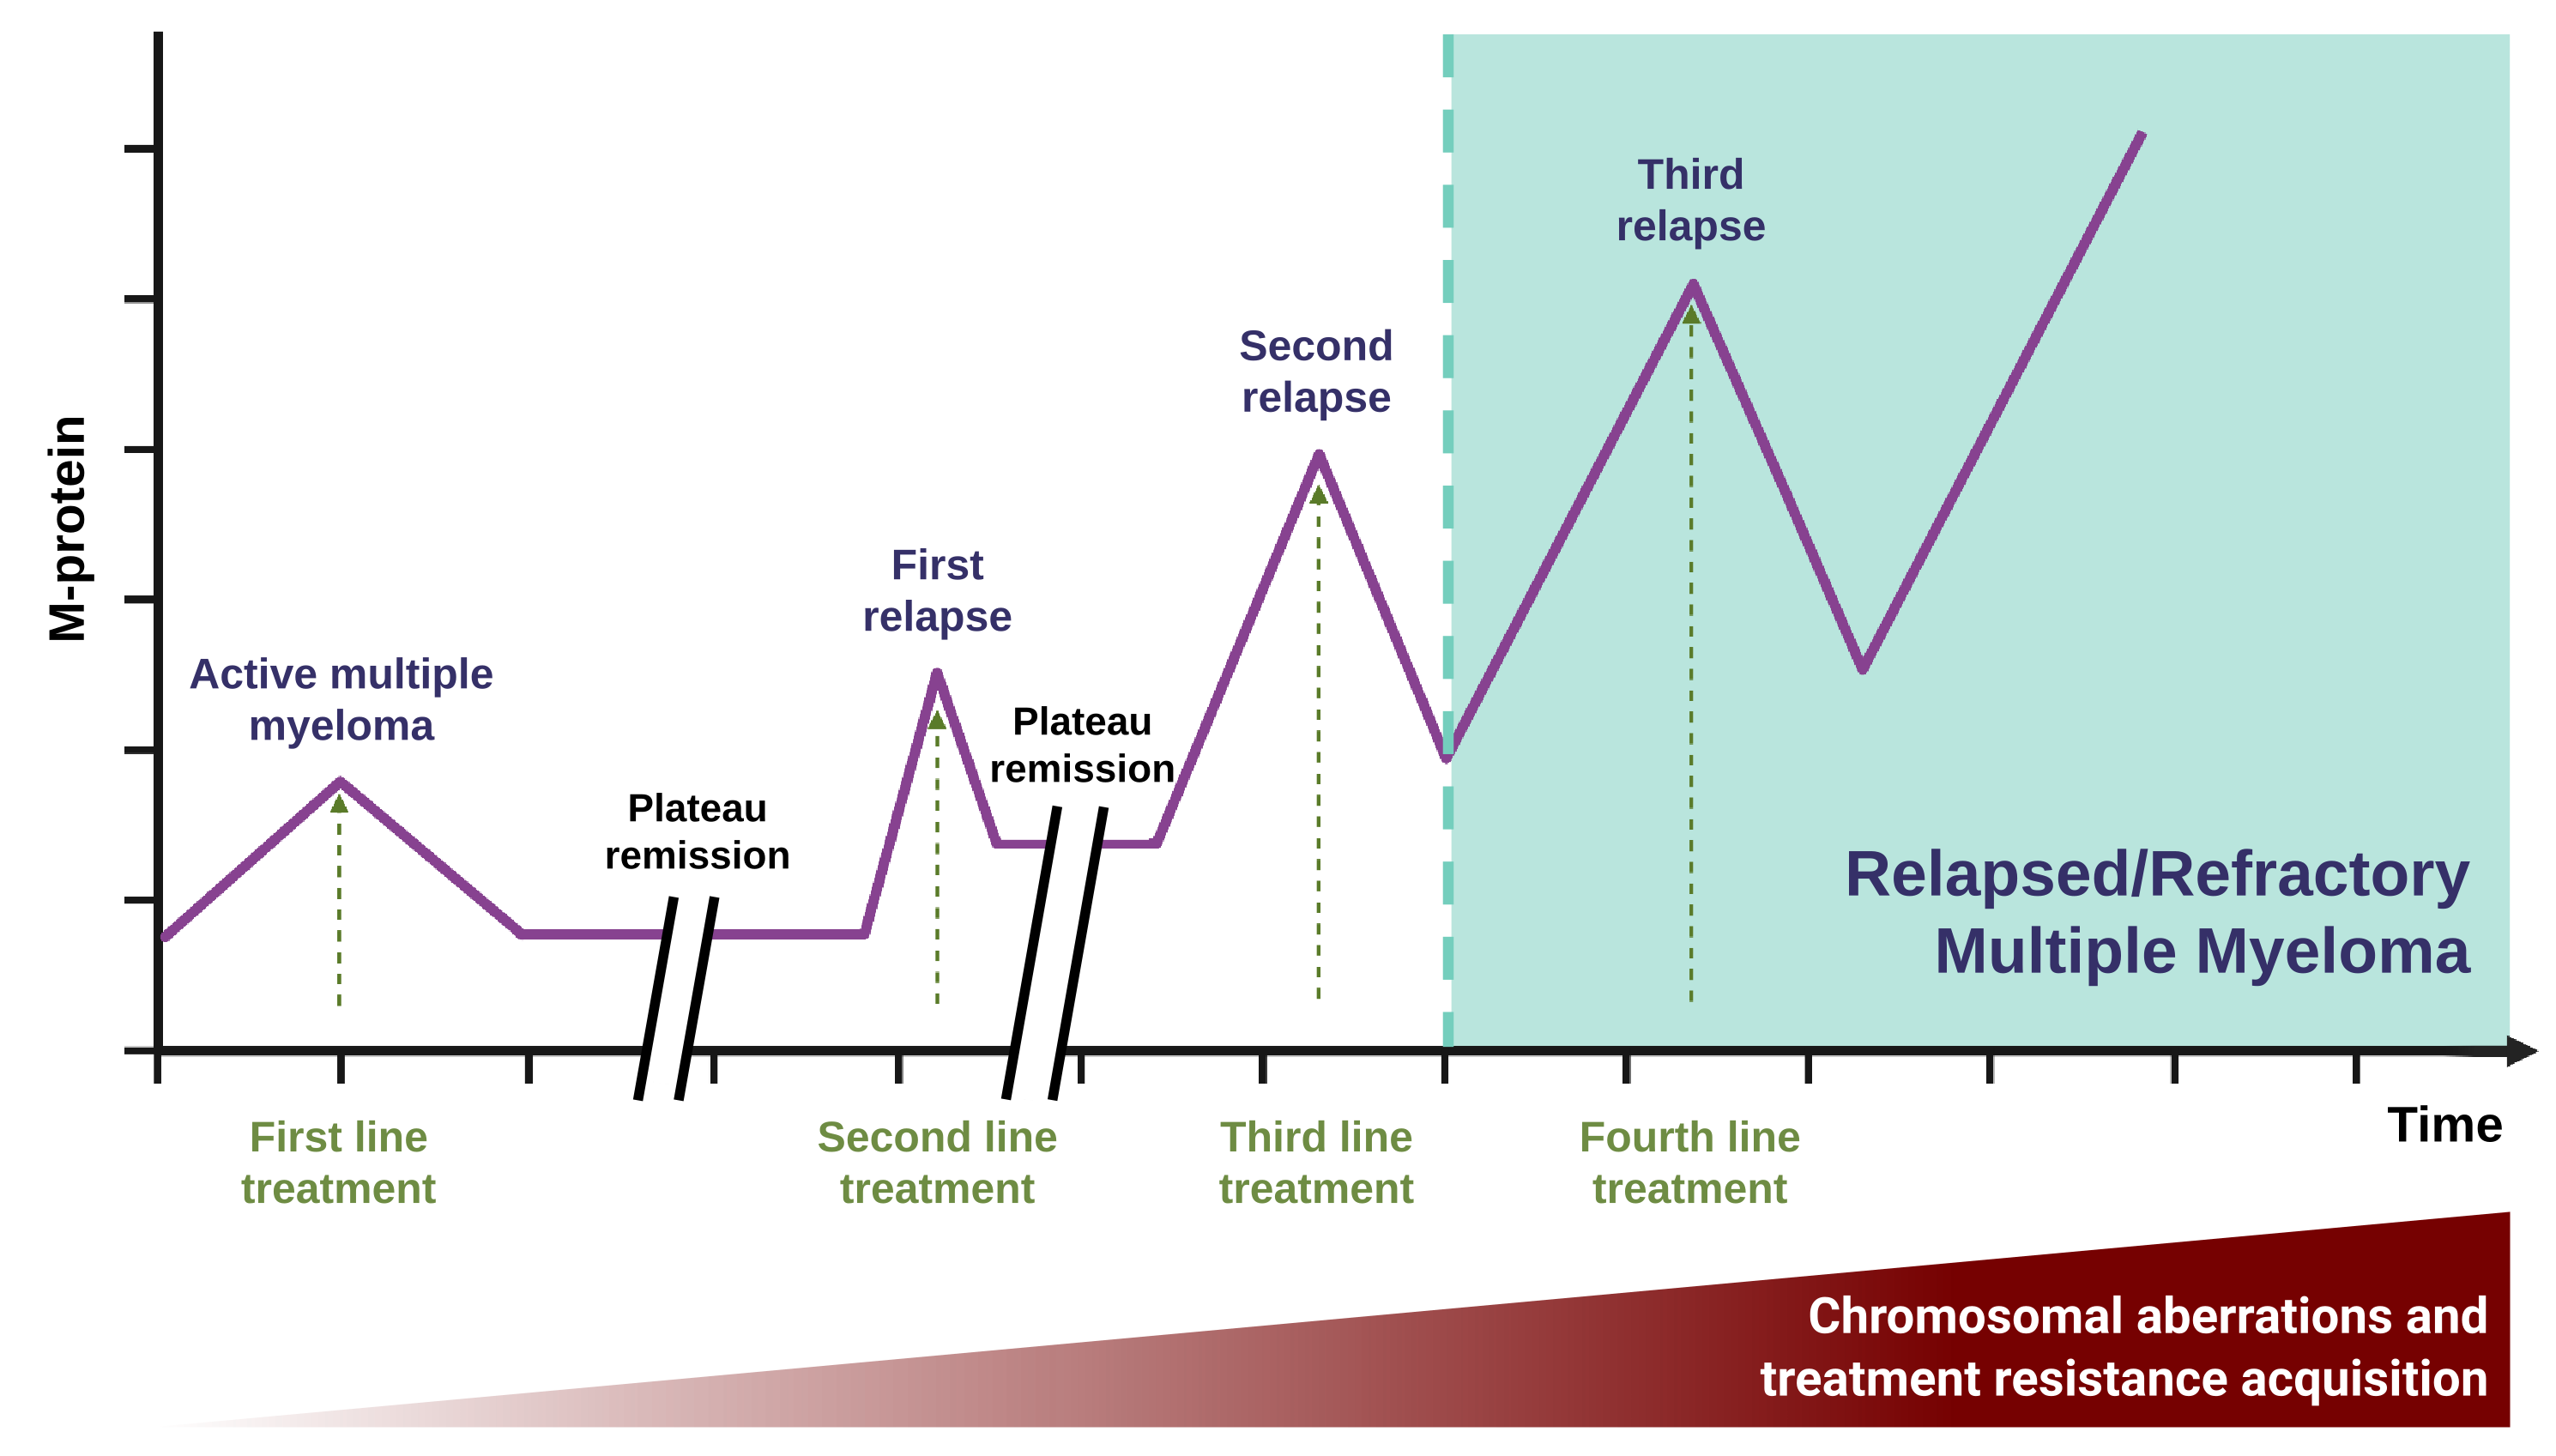
\includegraphics[width=0.8\textwidth]{img/evo_MM.png}
    \caption[Remission/relapse cycle of Multiple Myeloma]{Remission/relapse 
    cycle of MM. The disease trajectory is characterized by serial cycles of 
    response, remission, and relapse in the presence of treatment, typically 
    monitored through M protein levels (an abnormal antibody produced by 
    malignant plasma cells). Through successive relapses, MM cells acquire new 
    chromosomal abnormalities, leading to clonal evolution with diminished 
    depth and duration of response over time. Courtesy of Álvaro Otero Sobrino, 
    researcher of Hospital 12 de Octubre's Hematological Malignancies group.}
    \label{fig:evo_MM}
\end{figure}

    
    \chapter{Objetives}

The primary aim of this research is to evaluate cutting-edge long-read 
sequencing approaches to track and analyze somatic structural variations across 
cancer genomes evolution. To this end, we have established the following 
specific objectives:

\begin{enumerate}

    \item Assess the technical feasibility of detecting large-scale structural 
    variants using synthetic long-read sequencing data that simulates current 
    ONT flow cell protocols.
    
    \item Evaluate and compare current SV callers, considering both their 
    detection accuracy and computational efficiency, to identify 
    optimal solutions for analysis workflows.
    
    \item Validate the possibility of detecting clinically relevant Multiple 
    Myeloma markers using long-read sequencing approaches, identifying both 
    their potential and current limitations for clinical applications.
    
\end{enumerate}
    \blankpage{}

    \chapter{Materials and methods}

\section{Computing resources}

Code development for this project was performed on a VANT MOOVE15 laptop with an 
Intel\regsup{} Core™ i5-1235U processor, 64 GB DDR4 RAM, and 2 TB NVMe SSD, 
running Ubuntu 24.04.1 LTS.

Due to the computational demands of the tasks required to achieve the proposed
objectives, the CNIO High-Performance Computing (HPC) cluster was utilized. 
The cluster currently features 12 compute nodes with configurations as detailed 
in \textbf{Table \ref{tab:nodes}}.

\begingroup
\vspace{0.30cm}
\footnotesize

\begin{longtable}{>{\RaggedRight\arraybackslash}p{1.5cm} 
                  >{\RaggedRight\arraybackslash}p{2.5cm} 
                  >{\RaggedRight\arraybackslash}p{2cm}
                  >{\RaggedRight\arraybackslash}p{2cm}
                  >{\RaggedRight\arraybackslash}p{4cm}}
    \captionsetup{labelfont=bf, font=footnotesize}
    \caption[Technical specifications of computing nodes in CNIO's HPC cluster]
    {Technical specifications of computing nodes in CNIO's HPC cluster 
    \cite{noauthor_usage_nodate}.}\label{tab:nodes}\\
    
    \toprule
    \rowcolor{lightgray}
    \textbf{Count} & \textbf{Node names} & \textbf{CPU cores} & \textbf{RAM} & \textbf{GPUs} \\ 
    \midrule
    \endfirsthead
    
    \multicolumn{5}{@{}l}{\RaggedRight \textbf{\tablename\ \thetable{}} -- Continued} \\
    \\
    \toprule
    \rowcolor{lightgray}
    \textbf{Count} & \textbf{Node names} & \textbf{CPU cores} & \textbf{RAM} & \textbf{GPUs} \\ 
    \midrule
    \endhead
    \\
    \midrule 
    \multicolumn{5}{r}{\footnotesize Continued on next page} \\
    \endfoot
    
    \bottomrule
    \endlastfoot

    \\
    1     & bc001      & 24  & 32 GB  & -- \\
    \\
    6     & bc00[2-7]  & 52  & 512 GB & -- \\
    \\
    3     & bc00[8-10] & 128 & 1 TB   & -- \\
    \\
    1     & hm001      & 224 & 2 TB   & -- \\
    \\
    1     & gp001      & 112 & 768 GB & 3 x Nvidia A100 80 GB \\
    \\

\end{longtable}
\endgroup
    
The cluster's storage resources include 52 TB of standard storage space for 
user home directories, complemented by 512 TB of high-performance storage 
optimized for compute job input and output operations. From this 
high-performance storage, 30 TB was specifically allocated as project space 
for code execution and data generation.

\section{Software tools}

Visual Studio Code served as the primary interface for cluster access via SSH 
and code development. The implementation primarily utilized Bash, Python, and R 
programming languages.

The cluster operates under Slurm Workload Manager, a Linux/Unix-based system for 
HPC resource management. Workflow integration was accomplished through 
Snakemake, a Python-based workflow manager that enables isolated software 
environments for each workflow step using Conda, thus avoiding node-specific 
installations and potential compatibility issues.

Miniforge, a minimal Conda distribution preconfigured with conda-forge as the 
default software, was installed to manage Conda environments. The Bioconda 
software repository was added to access specialized bioinformatics packages.

A detailed compilation of all software tools utilized throughout this research
is presented in \textbf{Table~\ref{tab:software}}. The subsequent subsections 
detail how these tools were strategically integrated into comprehensive 
workflows to address the project's specific objectives.

\subsection{Simulating long-read data and SV calling}

In the absence of curated long-read gold-standard datasets, testing SV calling methods 
with real biological datasets demands complex experimental procedures that are 
time-consuming, expensive, and potentially biased. In contrast, \textit{in silico} 
approaches provide an efficient and accurate alternative to evaluate SV caller 
performance, where the ground truth is known.

\subsubsection{Data simulator}

VISOR toolkit was selected for haplotype-specific simulations of simple and 
complex SVs. Their VISOR LASeR module uses an error model trained on ONT R10.4.1 
reads from 2023, provided by Badread \cite{wick_badread_2019}.

\subsubsection{SV callers}

A set of SV calling tools was selected based on two key criteria: ONT 
long-read compatibility and somatic SV detection ability. Each selected caller 
provides distinct features valuable for this analysis:

\begin{itemize}[label=\tiny\raise.5ex\hbox{•}, leftmargin=\parindent]

    \item \textbf{SAVANA}: Implements a machine learning model trained on 
    tumor-normal paired samples to detect somatic SVs and copy number 
    aberrations (CNAs) in clinical cases.

    \item \textbf{Severus}: Specializes in tumor/normal comparative analysis, 
    supporting multi-tumor samples and employing breakpoint graph frameworks 
    for complex chromosomal rearrangement detection.

    \item \textbf{Sniffles2}: A pioneering ONT long-read SV caller since 2018, 
    maintaining continuous development and regular updates.

    \item \textbf{SVision-pro}: Employs a neural network-based approach that 
    converts genomic features from paired samples into image representations 
    for comparative SV detection.
    
\end{itemize}

\subsubsection{Generation and calling of SVs}

A comprehensive workflow for VISOR-based simulations and SV calling analysis was 
developed. The complete code and documentation are available in the following
repository: \url{https://github.com/villena-francis/visor-simulations}. 
\textbf{Figure \ref{fig:visor-sim}} illustrates the key workflow steps.

\newpage

\begin{figure}[H]
    \centering
    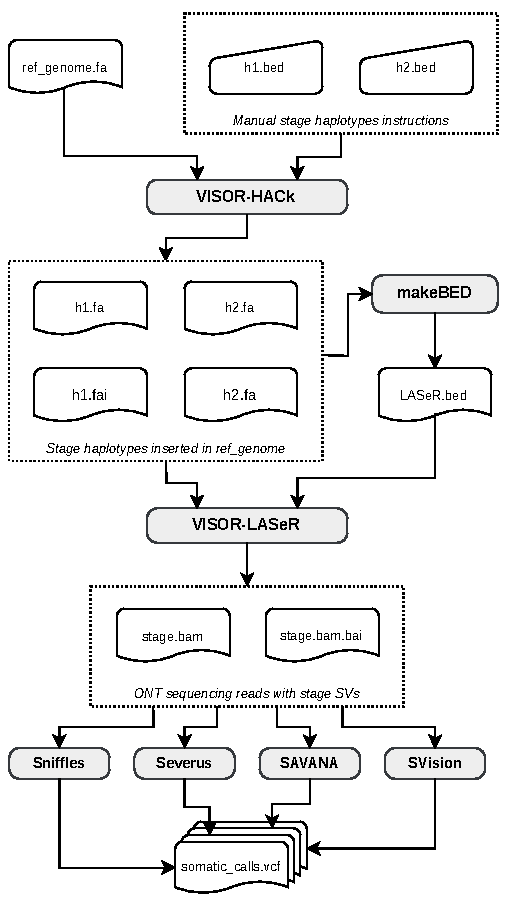
\includegraphics[scale=1.3]{img/visor-simulations.pdf}
    \caption[Simplified version of ``visor-simulations'' workflow for long-read 
    simulation and SV calling]{Simplified version of ``visor-simulations'' 
    workflow for long-read simulation and SV calling. VISOR-HACk generates FASTA 
    files (reference sequences) with incorporated SVs using a reference genome and 
    BED-formatted haplotype instructions (tab-delimited genomic coordinates). 
    The makeBED script creates a BED file (genomic intervals) from maximum 
    chromosome sizes extracted from haplotype FASTAs. VISOR-LASeR then generates 
    BAM files (aligned sequencing reads) and their indexes (.bai) using these 
    files as input. each generating its corresponding variant call file (VCF) 
    containing the identified SVs. The workflow parallelizes simulations 
    across stages using configuration files and wildcards, producing 
    multiple replicates at various sequencing coverages with corresponding 
    normal samples.}
    \label{fig:visor-sim}
\end{figure}

\subsubsection{Simulation stages}

Each stage incorporates specific SVs into the GRCh38 reference genome, simulated 
at four coverage levels: 30x, 50x, 100x, and 200x. The initial stage generated 
one normal sample and three tumor replicates per coverage level, totaling 16 BAM 
simulations. Subsequent stages reused the normal samples, requiring only 12 
simulations each through the automation provided by the ``visor-simulations'' 
workflow. 

The stage generated for this project (v1) incorporated six chromosomal 
aberrations characteristic of multiple myeloma, including tandem duplications, 
deletions, and various types of translocations (\textbf{Table~\ref{tab:stagesV1}}). 
Breakpoint coordinates for these structural variants were approximately 
determined using the UCSC Genome Browser, as specific locations were not 
detailed in the clinical literature.

\begingroup
\vspace{0.35cm}

\footnotesize

\begin{longtable}{>{\RaggedRight\arraybackslash}p{2.5cm} 
                  >{\RaggedRight\arraybackslash}p{10.5cm} 
                  >{\RaggedLeft\arraybackslash}p{1.75cm}}
    \captionsetup{labelfont=bf, font=footnotesize}
    \caption[Simulated chromosomal aberrations characteristic of Multiple 
    Myeloma]{\footnotesize Simulated chromosomal aberrations characteristic of 
    Multiple Myeloma \cite{aksenova_genome_2021}. Size values represent the final 
    length in base pairs (bp) after genome insertion. Tandem duplication 
    consists of a 2,030,586 bp fragment repeated four times. Input files for 
    VISOR read simulation available at 
    \url{https://github.com/villena-francis/visor-simulations/tree/main/resources/v1}}. 
    \label{tab:stagesV1}\\
    
    \toprule
    \rowcolor{lightgray}
    \textbf{SV type} & \textbf{Description} & \textbf{Size (pb)} \\ 
    \midrule
    \endfirsthead
    
    \multicolumn{3}{@{}l}{\RaggedRight \textbf{\tablename\ \thetable{}} -- Continued} \\
    \\
    \toprule
    \rowcolor{lightgray}
    \textbf{SV type} & \textbf{Description} & \textbf{Size (pb)} \\ 
    \midrule
    \\
    \endhead
    \\
    \midrule 
    \multicolumn{3}{r}{\footnotesize Continued on next page} \\
    \endfoot
    
    \bottomrule
    \endlastfoot

    \\
    Tandem \mbox{duplication}         & Amplification of chromosome 1q (1q21+), representing one of the most frequent structural cytogenetic abnormalities in Multiple Myeloma, occurring in approximately 40\% of cases .     & 10152930 \\
    \\
    Deletion                          & Deletion of chromosome 17p, present in approximately 10\% of Multiple Myeloma cases, serves as a significant poor prognostic indicator. The minimally deleted region at locus 17p13 encompasses the tumor suppressor gene TP53 & 234564 \\
    \\
    Translocation \mbox{(reciprocal)} & Chromosomal rearrangement involving the immunoglobulin heavy chain (IGH) gene at 14q32, a hallmark genetic event in Multiple Myeloma pathogenesis.                                                  & 1502367  \\
    \\
    Translocation \mbox{(cut-paste)}  & Rearrangement involving CDKN2A, a crucial tumor suppressor gene whose inactivation through mutations or deletions is among the most frequent alterations in human cancers, second only to TP53 alterations. & 31271 \\
    \\
    Translocation \mbox{(copy-paste)} & Structural variation affecting the KRAS oncogene region, whose alterations are frequently associated with Multiple Myeloma progression.  & 45683 \\
    \\
    Inversion                         & Chromosomal inversion at 6q25.1, included as a control variant to validate the detection capabilities of structural variant analysis pipelines, although not typically characteristic in Multiple Myeloma.          & 3600001  \\
    \\

\end{longtable}
\endgroup

\newpage 

\subsection{Benchmarking of SV callers}

\subsubsection{Data subsampling for local device processing}

Visual inspection of BAM file reads is essential for validating simulation 
quality and SV caller accuracy. Due to cluster limitations with graphical 
interfaces, this analysis requires local processing. We developed a workflow to 
split whole-genome BAM files by chromosome, available at 
\url{https://github.com/villena-francis/bam-splitter}. 
\textbf{Figure \ref{fig:bam-splitter}} illustrates the workflow's key 
components.

\begin{figure}[H]
    \centering
    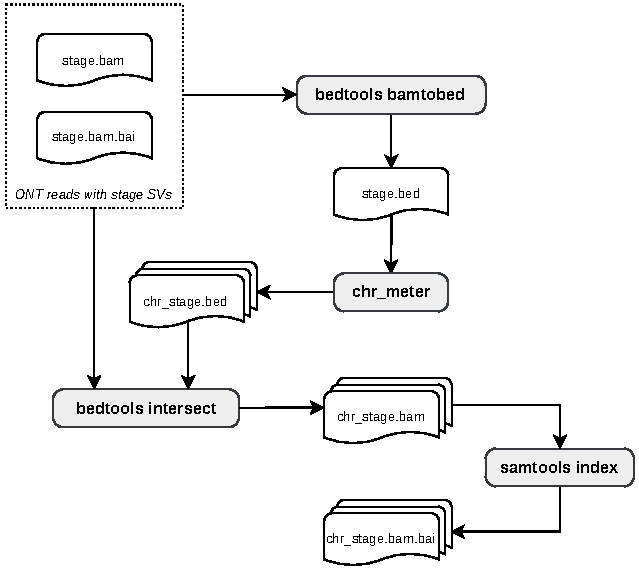
\includegraphics[scale=1.3]{img/bam-splitter.pdf}
    \caption[Simplified version of ``bam-splitter'' workflow for chromosomal 
    splitting of BAM files]{Simplified version of ``bam-splitter'' workflow for 
    chromosomal splitting of BAM files. The process begins with bedtools 
    bamtobed generating a comprehensive BED file of chromosome coordinates. 
    The chr\_meter script then creates individual BED files for selected 
    chromosomes, which bedtools intersect uses to produce chromosome-specific 
    BAM files. Samtools generates corresponding indexes for each BAM file. The 
    workflow employs configuration files and wildcards to parallelize chromosome 
    processing.}
    \label{fig:bam-splitter}
\end{figure}

\subsubsection{Visualization of long read alignments}

Chromosomal BED visualization was conducted using Genome-Wide (GW), an advanced, 
ultra-fast genome browser capable of exploring extensive genomic regions and 
complete chromosomes. GW's specialized features, particularly its VCF-based 
manual curation capability, facilitated rapid validation of SV caller 
predictions.

\subsubsection{Classification of SV calling results}

Performance evaluation of SV callers employed a binary classification framework 
with the following criteria:

\begin{itemize}[label=\tiny\raise.5ex\hbox{•}, leftmargin=\parindent]

    \item \textbf{True Positives (TP)}: Successfully detected simulated SVs.
    
    \item \textbf{False Positives (FP)}: Caller-identified SVs absent in 
    simulation, verified through read inspection.
    
    \item \textbf{False Negatives (FN)}: Simulated SVs present in reads but 
    undetected by caller.

\end{itemize}

True Negatives (TN) were excluded from this analysis due to their 
inapplicability in SV calling evaluation, given the vast genomic space and 
nature of SV detection methods.

\subsubsection{Metrics used}

Due to the impossibility of quantifying true negatives in SV calling, we 
employed TN-independent metrics:

\begin{enumerate}[leftmargin=\parindent]
    
    \item \textbf{Recall}: Proportion of correctly identified positive cases
    \begin{equation}
        \label{eq:recall}
        Recall = \frac{TP}{TP + FN}
    \end{equation}

    \item \textbf{Precision}: Accuracy of positive predictions
    \begin{equation}
        \label{eq:precision}
        Precision = \frac{TP}{TP + FP}
    \end{equation}

    \item \textbf{F1 Score}: Harmonic mean of precision and recall
    \begin{equation}
        \label{eq:f1score}
        F1 = 2 \cdot \frac{precision \cdot recall}{precision + recall}
    \end{equation}

\end{enumerate}

Computational efficiency was evaluated using Slurm-generated statistics: CPU/GPU 
utilization (cores), RAM consumption (GB), and execution time (minutes).

\subsubsection{Data Visualization and Statistical Analysis}

Metric analysis and visualization were implemented through R scripts available 
at \url{https://github.com/villena-francis/master_thesis/tree/main/data/cluster_bmk}.









    \chapter{Results}

\section{Simulated data}

VISOR simulations generated a total of 14 TB of simulated ONT long-read 
sequencing data. Of this volume, approximately 5.6 TB corresponded to reference 
genome-aligned reads in BAM format and their respective indices, while the 
remaining data volume consisted of unaligned reads in FASTQ format 
(\textbf{Table~\ref{tab:file_sizes}}). The computational resources required for 
the simulation process were monitored, with CPU utilization, RAM consumption, 
and generation times detailed in \textbf{Figure~\ref{fig:hpc_visor_laser}}.

\begin{figure}[H]
    \centering
    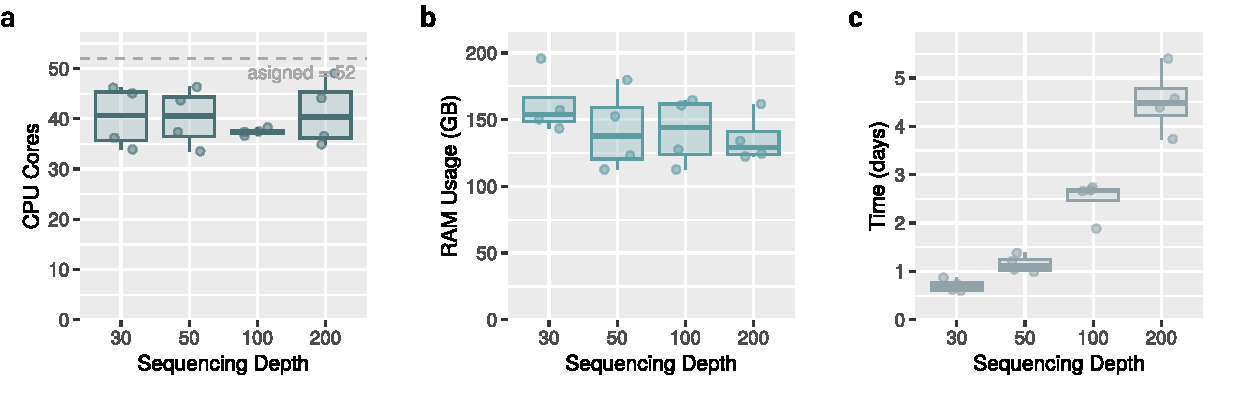
\includegraphics[width=\textwidth]{data/cluster_bmk/hpc_visor_laser.pdf}
    \caption[Computational resources demand of VISOR LASeR module]{Computational 
    resources demand of VISOR LASeR module by sequencing depth, which represents 
    the simulation bottleneck due to its CPU cores (\textbf{a}) and RAM memory 
    (\textbf{b}) consumption over time (\textbf{c}). For each sequncing deph, 
    three ``tumour'' and one ``normal'' WGS technical replicas were obtained 
    by simulating long reads. Calculations for VISOR HACk module were not 
    performed since it runs only once for a few minutes with low resource 
    consumption to introduce the SV set into the reference genome that will 
    feed VISOR LASeR. The raw data used for all calculations is available in REPO.}
    \label{fig:hpc_visor_laser}
\end{figure}

\section{SV calling}

SV callers generate VCF files similar to those produced by SNV callers. However, 
in SV calling, each row represents a breakpoint, which defines the boundary of a 
structural variant. Simple SVs, such as insertions or deletions, require the 
identification of two breakpoints, while complex variants like reciprocal 
translocations necessitate the detection of four breakpoints. To illustrate the 
final output files generated by each caller, results from a 50x coverage 
simulated sample are available at 
\url{https://github.com/villena-francis/master_thesis/tree/main/data/vcf_examples}.

\subsubsection{Standard VCF Outputs}

\begin{itemize}

\item \textbf{SAVANA}. A significant limitation in SAVANA's VCF output, compared 
to other variant callers, is its inability to classify SV types. The tool only 
identifies and correlates breakpoints without providing information about the 
specific type of SV present. 

\item \textbf{Severus}. Beyond conventional SV detection, 
Severus incorporates specialized processing for variable number tandem repeats 
(VNTRs), enabling precise annotation of structural variants within these regions. 
The tool provides comprehensive output including standard VCF files, detailed 
quality metrics in log files, and graphical representations of chromosomal 
rearrangements through visualization plots.

\item \textbf{Sniffles2}. This caller generates standard VCF output exclusively, 
without additional supporting files or visualizations.

\item \textbf{SVision-pro}: Despite leveraging an innovative image-based 
encoding approach to analyze genomic features and detect inter-genome variations 
between tumor-normal paired samples, SVision-pro's output is limited to standard 
VCF files. The visual representations used in its internal processing pipeline 
are not accessible in the final output.

\end{itemize}

\subsection{Computational demands}

While computational requirements for analyzing real samples may be higher due to 
the larger number of SVs typically detected in actual cancer genomes, our 
simulation-based analysis provides proportional estimates of computational 
demands across different sequencing coverages for each of the four callers 
evaluated. Core utilization, RAM consumption, and execution times are 
illustrated in \textbf{Figure~\ref{fig:hpc_calls}}.

A key distinction in processing unit allocation lies with SVision-pro, whose 
neural network-based SV detection model is GPU-optimized, whereas SAVANA, 
Severus, and Sniffles2 rely on CPU-based computation. We allocated 24 cores to 
GPU-based callers, as preliminary testing showed peak utilization remained 
below 20 cores.

The initial RAM allocation of 40 GB proved sufficient for Severus, Sniffles2, 
and SVision-pro, with memory usage increasing linearly with sequencing depth. 
However, SAVANA consistently exceeded this limit across all 
sequencing coverages, demonstrating significantly higher memory requirements 
compared to other callers.

SVision-pro demonstrates the lowest execution times across all sequencing 
depths, followed closely by Sniffles2. Both callers show efficient performance 
scaling, with execution times increasing sub-linearly with sequencing depth. 
SAVANA shows the highest execution times at the three lower sequencing 
coverages (30x, 50x and 100x), while Severus requires the longest processing 
time at maximum coverage (200x).

\begin{figure}[H]
    \centering
    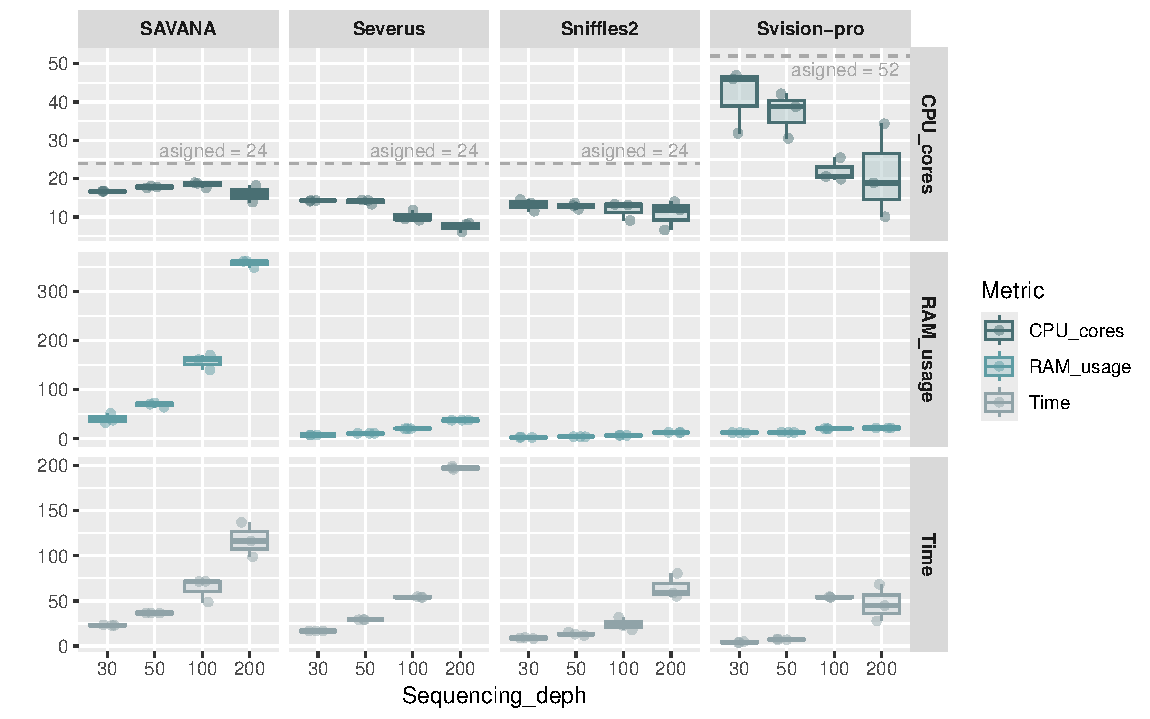
\includegraphics[width=\textwidth]{data/cluster_bmk/hpc_calls.pdf}
    \caption[Computational resource demanded for SV detection methods]{
    Computational resources demanded for SV detection methods of SAVANA, 
    Severus, Sniffles2, and SVision-pro, measured in CPU cores, RAM memory (GB), 
    and execution time (minutes). For each sequencing depth, three measurements 
    per metric were obtained by comparing a single normal sample against three
    technical replicates of the tumor sample. The complete raw data used for
    all calculations is available in 
    \url{https://github.com/villena-francis/master_thesis/tree/main/data/cluster_bmk/hpc_data}.}
    \label{fig:hpc_calls}
\end{figure}

\subsection{Calling performance}

From the proposed SVs in synthetic data, SAVANA and Severus successfully identified 
all instances of tandem duplication, deletion, inversion, and reciprocal 
translocation. Although cut-paste and copy-paste translocations were included in 
the simulation instructions, only the deletion component of cut-paste events was 
successfully reconstructed in the BAM files, while the translocation component and 
copy-paste events failed to be reconstructed.In contrast, neither Sniffles2 nor 
SVision-pro detected any of the simulated SVs, explaining the stark differences 
in Precision, Recall, and F1 scores shown in \textbf{Figure~\ref{fig:perform_calls}}. 


Visual inspection through GW of VISOR-generated BED files confirmed the presence 
of SVs detected by SAVANA and Severus, while validating the absence of 
undetected variants. This verification ruled out false negatives, resulting in a 
recall of 1.0 for both callers. Notably, Severus reported additional findings 
from its specialized VNTR analysis, which, although not explicitly introduced in 
simulation instructions, were present as artifacts from VISOR-LASeR's error 
model.

While SAVANA and Severus achieved identical recall values, SAVANA demonstrates 
higher precision due to Severus reporting slightly more false positives. Despite 
generating significantly more variant calls than both SAVANA and Severus, 
neither Sniffles2 nor SVision-pro detected any of the expected simulated SVs. 
Extensive visual inspection of their findings revealed no overlap with validated 
variants, resulting in their classification as false positives and consequently 
zero precision scores.

As a balanced measure combining precision and recall, F1 score reflects the 
overall performance of each caller. SAVANA achieves the highest F1 score due to 
its perfect recall and superior precision. Severus follows closely, with its 
slightly lower F1 score attributed solely to its marginally higher false 
positive rate, as it maintained perfect recall. Both Sniffles2 and SVision-pro 
yield F1 scores of zero, as expected from their complete absence of true 
positive findings and high number of false positive calls.

\begin{figure}[H]
    \centering
    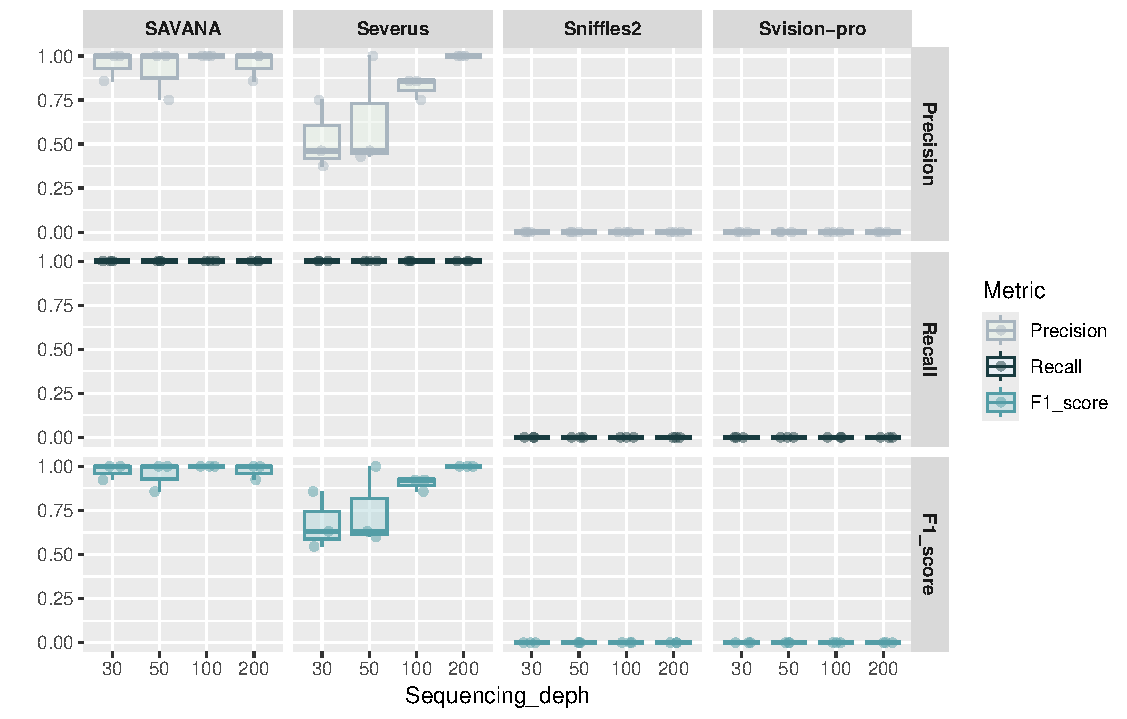
\includegraphics[width=\textwidth]{data/cluster_bmk/perform_calls.pdf}
    \caption[Performance of evaluated SV calling methods]{Performance of SV calling
    methods of SAVANA, Severus, Sniffles2 and SVision-pro, based on precision, 
    recall, and F1 score metrics. For each sequencing depth, three results per 
    metric were obtained by comparing one normal sample against three technical 
    replicates of the tumor sample. The raw data used for all calculations is 
    available in 
    \url{https://github.com/villena-francis/master_thesis/tree/main/data/cluster_bmk/calls_data}.}
    \label{fig:perform_calls}
\end{figure}
    
    \chapter{Discussion}

\section{Computational and Resource Requirements}

The synthetic data analysis configuration in this project demanded substantial 
computational resources: 14 TB of storage (2.73\% of CNIO's HPC cluster 
capacity) and 832 cores for VISOR-LASeR execution (52 cores per sample, 
exceeding 114\% of available cores). Furthermore, the single-job-per-GPU 
restriction for SVision-pro execution led to extended processing times. This 
intensive resource utilization presented significant challenges given the 
cluster's shared nature among multiple CNIO research groups and projects.
These findings emphasize that computational tool selection should consider not 
only accuracy but also efficient resource management based on available 
computing resources as critical evaluation criteria.

\section{Simulation Design and Parameters}

The selection of SVs for simulation was influenced by ongoing research in the 
CNIO Bioinformatics Unit's long-reads group, specifically their collaboration 
with Hospital 12 de Octubre's Hematological Malignancies group on WGS of MM 
patient samples, comparing pre-treatments and relapses. Consequently, the SV 
set includes both characteristic MM variants and more speculative cancer-related 
SVs to cover a broader spectrum of SVs. Despite the availability of 
T2T genomes, GRCh38 was chosen as the reference genome due to its extensive use 
in research and the substantial accumulation of annotation-associated findings 
throughout its trajectory.

The SV simulation was configured to represent bulk sequencing of a homogeneous 
cell population containing a single clone, with all variant allele frequencies 
(VAFs) set to 0.5. This configuration ensures variants are present on one allele 
and represented in half of the generated sequencing reads. Such design aimed to 
provide clear variant representation in the reads, theoretically ensuring 
reliable detection by callers while facilitating visual validation through GW. 
However, this idealized scenario differs from real tumor samples, where variant 
allele frequencies can vary significantly due to tumor heterogeneity and normal 
cell contamination \cite{dagogo-jack_tumour_2018}.

Reads were simulated with a mean length of 15,000 bp and a standard deviation of 
13,000 bp, using VISOR-LASeR default settings. These parameters align with 
realistic values obtainable through actual sequencing using the PromethION 
platform's protocol for 10 kb human DNA with Ligation Sequencing Kit V14 
\cite{noauthor_ligation_2022}, which has been selected for sequencing the MM
patient samples. Notably, this protocol aims to generate $\sim$30-40x genome 
coverage. Our benchmarking results at higher coverages (100x and 200x) showed 
no substantial performance improvements for any caller in detecting simulated 
SVs, suggesting that the additional costs and efforts associated with using 
multiple flow cells and preparing larger sample quantities may not be justified. 
However, Severus detected unplanned VNTR anomalies at lower coverages (30x and 50x), 
introduced by the Badread error model trained on ONT R10.4.1 reads. This 
observation is crucial for real sample sequencing: while such artifacts were 
more prevalent in R9.4 reads (see \textbf{Figure \ref{fig:ont_pores}}), 
they might still influence SV calling results, as even a small number of reads 
containing these sequencing artifacts could be considered representative by 
callers at the coverage levels currently achievable with a single flowcell.

\section{SV Caller Performance and Limitations}

Performance metrics position SAVANA as the top performer, yet its limitation to 
breakpoint correlation without SV classification represents a significant 
drawback. This limitation, combined with substantially higher RAM consumption 
and execution times compared to other callers, impacts its practical utility. 
Severus, despite slightly lower precision, matches SAVANA's recall while 
maintaining lower RAM usage and provides comprehensive SV classification 
alongside visual representations of chromosomal rearrangements. These 
characteristics likely influenced Severus's integration into the latest EPI2ME 
release, Oxford Nanopore's open-source platform designed to provide wet lab 
scientists with a user-friendly interface for data analysis without requiring 
advanced bioinformatics skills. However, despite its integration, EPI2ME's 
documentation lacks comparative analyses justifying Severus's selection over 
other SV callers, possibly due to its target audience 
\cite{oxford_nanopore_technologies_epi2me_nodate}.

Our evaluation employed minimum argument sets for all callers, relying on 
developer-configured default parameters for complex adjustments. This 
standardized approach may explain the poor performance of Sniffles2 and 
SVision-pro, particularly in detecting large SVs, as default settings might not 
be optimized for such variants. Notably, following our analysis, Sniffles2 
version 2.5 released improvements specifically targeting detection of large 
deletions and duplications ($>$ 50 kb) \cite{noauthor_releases_nodate}. 
Interestingly, the better-performing tools in our analysis (SAVANA and Severus) 
remain available only in preprint servers, while Sniffles2 and SVision-pro are 
published in peer-reviewed journals.

\section{Clinical Relevance and Technical Challenges}

VISOR toolkit proved valuable for evaluating SV callers' capability to identify 
characteristic large structural events in Multiple Myeloma using ONT long reads, 
particularly those with diagnostic significance. Through synthetic data 
generation, we successfully validated the detection of two of the most frequent 
chromosomal aberrations in Multiple Myeloma, notably the largest SVs in our 
simulation set, using SAVANA and Severus: the tandem amplification of 1q21+ 
(100 Mb) and an IGH-involving translocation (1,5 Mb). These structural variants, 
currently verified in clinical settings through FISH due to the limitations of 
short-read sequencing assembly, represent critical diagnostic markers that could 
potentially be identified through long-read sequencing approaches.

The inability to simulate certain SVs provides valuable insights into technical 
limitations. While VISOR-HACk module unambiguously inserts all chromosomal 
abnormalities into a FASTA file using BED-formatted instructions and the 
reference genome as a template, challenges emerge in the VISOR-LASeR module,
which generates and aligns reads to the reference genome using minimap2. These 
limitations manifest in two ways: standard read lengths may be insufficient for 
reconstructing certain events, suggesting the potential need for ultra-long read 
protocols capable of generating sequences up to 4 Mb, and minimap2 alignment 
accuracy may be compromised for complex variants. For instance, in the 
copy-paste translocation designed to generate a proximal KRAS duplicate, the 
aligner appears to have defaulted to mapping all reads to the original gene 
position. Similarly, for the cut-paste translocation, only the deletion 
component was detected, while the inverted sequence insertion failed to be 
properly positioned, leaving its corresponding reads unaccounted for in the 
alignment.

\section{Visualization Tools and Challenges}

Initial visualization attempts of synthetic data were made using the 
widely-adopted Integrative Genomics Viewer (IGV) version 2.17.3. However, 
despite using chromosome-specific BAM files generated through the ``bam-splitter'' 
workflow, IGV's performance proved inadequate, exhibiting slow loading times and 
frequent crashes. Through email correspondence, Severus's lead developer shared 
similar experiences with long-read BAM files in IGV, suggesting a workaround of 
generating smaller BAM files containing only the SV regions with 1 Mb upstream 
and downstream sequences. While this approach would have been feasible for 
planned SVs, it proved impractical for investigating additional findings like 
VNTR anomalies due to automation limitations.

GW emerged as a capable alternative, efficiently handling both individual 
chromosome and whole-genome BAM files. Its VCF compatibility created an 
interactive index for rapid SV coordinate navigation, dramatically accelerating 
event verification. However, GW requires terminal-based operation in conjunction 
with an alignment view display, demanding more advanced computational skills 
compared to IGV's graphical user interface \textbf{Figure~\ref{fig:GW_UI}}. 
Nevertheless, GW's developer demonstrated strong responsiveness to error reports 
and feature requests through Github. Our project-specific experience led to 
reporting Conda installation \cite{noauthor_error_nodate} and loading genome
anotation files \cite{noauthor_display_nodate} issues, and requesting vector 
format export capabilities for alignment visualizations 
\cite{noauthor_saving_nodate}.

\section{Future Directions}

The development of robust tools for SV analysis in cancer genomes requires 
extensive testing and validation. While this study evaluated SV detection 
capabilities using synthetic data across different sequencing coverages, 
it primarily demonstrates the value of generating simulated datasets for 
benchmarking existing tools, developing new algorithms, and training machine 
learning models. These computational advances ultimately contribute to 
improving cancer genomics analysis in clinical settings.

A primary challenge lies in identifying structural events that, despite 
existing in the template genome, remained undetected in alignments. The 
unaligned reads in FASTQ format will be valuable for expanding benchmarks to 
include long-read aligners beyond minimap2, enabling more comprehensive tool 
evaluation. This expansion is crucial for improving the reliability of genomic 
analysis in clinical settings.

To enhance the exploration of SVs in cancer, future work should investigate 
several key aspects. First, examining the impact of read length on Sniffles2 and 
SVision-pro's calling capabilities, starting with sizes successfully identified 
in their published work. Second, introducing tumor heterogeneity through 
multiple clone combinations in synthetic sequencing data would better reflect 
real tumor complexities and allow evaluation of how varying VAFs affect SV 
detection capabilities. Third, exploring ultra-long read protocol parameters 
could help reconstruct previously undetected SVs. Based on our findings and 
resource efficiency considerations, these tests could focus on 30x and 50x 
sequencing coverages, aligning with practical clinical sequencing depths.

Data collection automation represents another critical area for improvement in 
clinical implementation. Currently, computational performance statistics are 
manually extracted from Slurm logs, a time-consuming process that could be 
streamlined through automated scripts. In anticipation of future evaluations, 
we have requested VISOR toolkit enhancements to log all parameters, both 
specified and default, facilitating automated tracking of simulation 
characteristics \cite{noauthor_add_nodate}. Additionally, The implementation of 
Truvari, a comprehensive toolkit for benchmarking, merging, 
and annotating structural variants from VCF files, would enhance the workflow
\cite{english_truvari_2022}. Its capabilities make it 
particularly suitable for analyzing tumor genome evolution through longitudinal 
sequencing and SV calling analysis.

Continuous communication with tool developers remains essential for optimizing 
clinical applications, sharing synthetic data experiences, and facilitating 
potential improvements. In this context, frequent requests for GW enhancements, 
particularly regarding data visualization and high-quality figure export 
capabilities, will support better clinical result interpretation and 
documentation.

Most critically, the experience gained through synthetic data analysis must be 
validated on ONT-sequenced tumor-normal paired patient samples, integrating 
structural variation analysis with SNVs and methylation data. This comprehensive 
genomic characterization approach aims to provide clinicians with more accurate 
and complete information for personalized cancer treatment decisions, ultimately 
improving patient outcomes through better-informed therapeutic strategies.


    \chapter{Conclusions}

Experimental data is essential for creating and improving computational methods, 
whose outputs not only provide new knowledge but can also serve as a foundation 
for refining future experiments. Synthetic data can catalyze this cycle, 
generating information faster and with fewer resource expenditures. Based on the 
results of this work, we can conclude the following:

\begin{enumerate}

    \item Long-read WGS data obtainable with a single ONT PromethION flow cell 
    with quality achievable from a single enables the reconstruction of 
    large-scale SVs, including insertions, deletions, translocations, and inversions 
    spanning complete chromosomal bands.
    
    \item Severus emerges as a balanced solution for SV detection, combining 
    comprehensive variant classification capabilities with efficient resource 
    utilization, making it suitable for routine analysis workflows.
    
    \item Long-read sequencing has the potential detect of clinically 
    significant MM markers, promising to enhance current diagnostic capabilities 
    despite some technical limitations in SV detection that remain to be addressed

\end{enumerate}

These findings provide valuable guidance for SV detection implementation while 
establishing a framework for synthetic data generation that can be used to 
benchmark tools and train future machine learning models. This work also 
highlights areas requiring further development in long-read sequencing analysis.

% \chapter{Conslusions}

% Los datos experimentales son una fuente imprescindible con los que crear o 
% mejorar métodos computacionales, cuyos outputs además de ofrecer nuevo 
% conocimiento pueden ser base para el perfeccionamiento de futuros experimentos.
% Los datos sintéticos pueden catalizar este ciclo, generando información más 
% rápido y con menor gasto de recursos. En base a los resultados de este trabajo, 
% podemos concluir lo siguiente:

% \begin{enumerate}

%     \item A partir de lecturas largas con la calidad obtenible a partir de una
%     WGS con una sola flowcell R 10.4.1 es posible reconstruir grandes 
%     inserciones delecciones, traslocaciones o inversiones que abarcan bandas 
%     cromosómicas completas.  

%     \item El método de SV calling de Severus es a balanced solution, offering 
%     comprehensive SV classification with reasonable resource consumption

%     \item The study validated the detection of clinically relevant Multiple 
%     Myeloma markers using long-read sequencing, demonstrating potential for 
%     clinical applications while identifying specific technical limitations

% \end{enumerate}

% These insights provide valuable guidance for implementing SVs detection in
% long-read sequencing in clinical settings while highlighting areas requiring 
% further development.

    \blankpage{}

    \printbibliography
    \blankpage{}

    \appendix
    \setcounter{figure}{0} % Reboot fig count
    \setcounter{table}{0}  % Reboot table count
    \renewcommand{\thechapter}{A}
\chapter{Appendix}

\begingroup
\footnotesize
\begin{longtable}{>{\RaggedRight\arraybackslash}p{3.5cm} >{\RaggedRight\arraybackslash}p{9.25cm} >{\RaggedRight\arraybackslash}p{2cm}}
    \captionsetup{labelfont=bf, font=footnotesize}
    \caption[Software tools used in this work]{\RaggedRight \footnotesize Software tools used in this work.}
    \label{tab:software}\\
    
    \toprule
\rowcolor{lightgray}
\textbf{Name} & \textbf{Source} & \textbf{Reference} \\ 
\midrule
\endfirsthead

\multicolumn{3}{@{}l}{\RaggedRight \tablename\ \thetable{} -- Continued} \\
\\
\toprule
\rowcolor{lightgray}
\textbf{Name} & \textbf{Source} & \textbf{Reference} \\ 
\midrule \\
\endhead \\
\midrule 
\multicolumn{3}{r}{\footnotesize Continued on next page} \\
\endfoot

\bottomrule
\endlastfoot

\\
Visual Studio Code v1.93.1   & \url{https://github.com/microsoft/vscode}          & --                                    \\
\\
Snakemake v8.29.6            & \url{https://github.com/snakemake/snakemake}       & \cite{koster_snakemakescalable_2012}  \\
\\
Miniforge v24.7.1            & \url{https://github.com/conda-forge/miniforge}     & --                                    \\
\\
VISOR v1.1.2.1               & \url{https://github.com/davidebolo1993/VISOR}      & \cite{bolognini_visor_2020}           \\
\\
minimap2 v2.28               & \url{https://github.com/lh3/minimap2}              & \cite{li_minimap2_2018}               \\          
\\
SAMtools v1.21               & \url{https://github.com/samtools/samtools}         & \cite{danecek_twelve_2021}            \\
\\
SAVANA v1.2.2                & \url{https://github.com/cortes-ciriano-lab/savana} & \cite{elrick_savana_2024}             \\
\\
Severus v1.2                 & \url{https://github.com/KolmogorovLab/Severus}     & \cite{keskus_severus_2024}            \\
\\
Sniffles2 v2.4               & \url{https://github.com/fritzsedlazeck/Sniffles}   & \cite{smolka_detection_2024}          \\
\\
SVision-Pro v2.0             & \url{https://github.com/sonGBowang125/SVision-pro} & \cite{wang_novo_2024}                 \\
\\
BEDtools v2.31.1             & \url{https://github.com/arq5x/bedtools2}           & \cite{quinlan_bedtools_2010}          \\
\\
GW v1.1.1                    & \url{https://github.com/kcleal/gw   }              & \cite{cleal_gw_2024}                  \\
\\
UCSC Genome Browser v2024    & \url{https://genome.ucsc.edu/index.html}           & \cite{perez_ucsc_2025}                \\
\\
Rstudio v2024.04.2           & \url{https://github.com/rstudio/rstudio}           & --                                    \\      
\\

\end{longtable}
\endgroup


\begingroup
\vspace{0.35cm}
\footnotesize
\begin{longtable}{>{\RaggedRight\arraybackslash}p{3.5cm} >{\RaggedRight\arraybackslash}p{2cm} >{\RaggedRight\arraybackslash}p{2cm} >{\RaggedRight\arraybackslash}p{2cm}}
    \captionsetup{labelfont=bf, font=footnotesize}
    \caption[File sizes by coverage]{\RaggedRight \footnotesize Size in gigabytes 
    of long-read sequencing files generated using VISOR toolkit at different 
    sequencing depths. The files include BAM, their indexes (BAI), and 
    unaligned reads in FASTQ files.}
    \label{tab:file_sizes}\\
    
    \toprule
    \rowcolor{lightgray}
    \textbf{Coverage} & \textbf{BAM} & \textbf{BAI} & \textbf{FASTQ} \\ 
    \midrule
    \endfirsthead
    
    \multicolumn{4}{@{}l}{\RaggedRight \tablename\ \thetable{} -- Continued} \\
    \\
    \toprule
    \rowcolor{lightgray}
    \textbf{Coverage} & \textbf{BAM} & \textbf{BAI} & \textbf{FASTQ} \\ 
    \midrule
    \endhead
    
    \midrule 
    \multicolumn{4}{r}{\footnotesize Continued on next page} \\
    \endfoot
    
    \bottomrule
    \endlastfoot
    
    30x\_normal & 112.42 & 0.0347 & 173.17 \\
    30x & 113.20 & 0.0351 & 174.02 \\
    30x & 113.19 & 0.0350 & 174.02 \\
    30x & 113.22 & 0.0350 & 174.02 \\
    50x\_normal & 187.01 & 0.0551 & 288.58 \\
    50x & 188.71 & 0.0556 & 289.99 \\
    50x & 188.85 & 0.0556 & 289.99 \\
    50x & 188.70 & 0.0556 & 289.99 \\
    100x\_normal & 374.24 & 0.1060 & 577.11 \\
    100x & 377.85 & 0.1071 & 579.93 \\
    100x & 377.86 & 0.1071 & 579.92 \\
    100x & 377.72 & 0.1071 & 579.93 \\
    200x\_normal & 748.34 & 0.2079 & 1157.12 \\
    200x & 754.99 & 0.2099 & 1157.12 \\
    200x & 754.89 & 0.2099 & 1157.12 \\
    200x & 755.35 & 0.2099 & 1157.12 \\
    \midrule
    \textbf{Total} & 5726.54 & 1.6266 & 8219.22 \\

\end{longtable}
\endgroup


\begin{figure}[H]
    \centering
    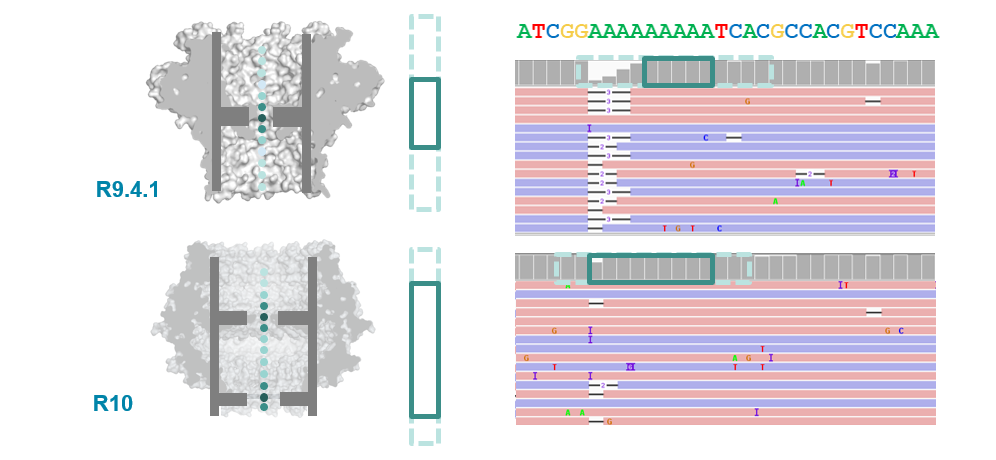
\includegraphics[width=\textwidth]{img/ont_pores.png}
    \caption[R10 nanopore improvements over R9]{The R10 nanopore design introduces 
    key improvements over its R9 predecessor: a longer barrel and dual reader head 
    architecture. These structural enhancements enable improved resolution of 
    homopolymeric regions such as VNRTs, significantly increasing the consensus 
    accuracy of nanopore sequencing data. Reproduced from 
    \cite{oxford_nanopore_technologies_r103_2020}.}
    \label{fig:ont_pores}
\end{figure}


\begin{figure}[H]
    \centering
    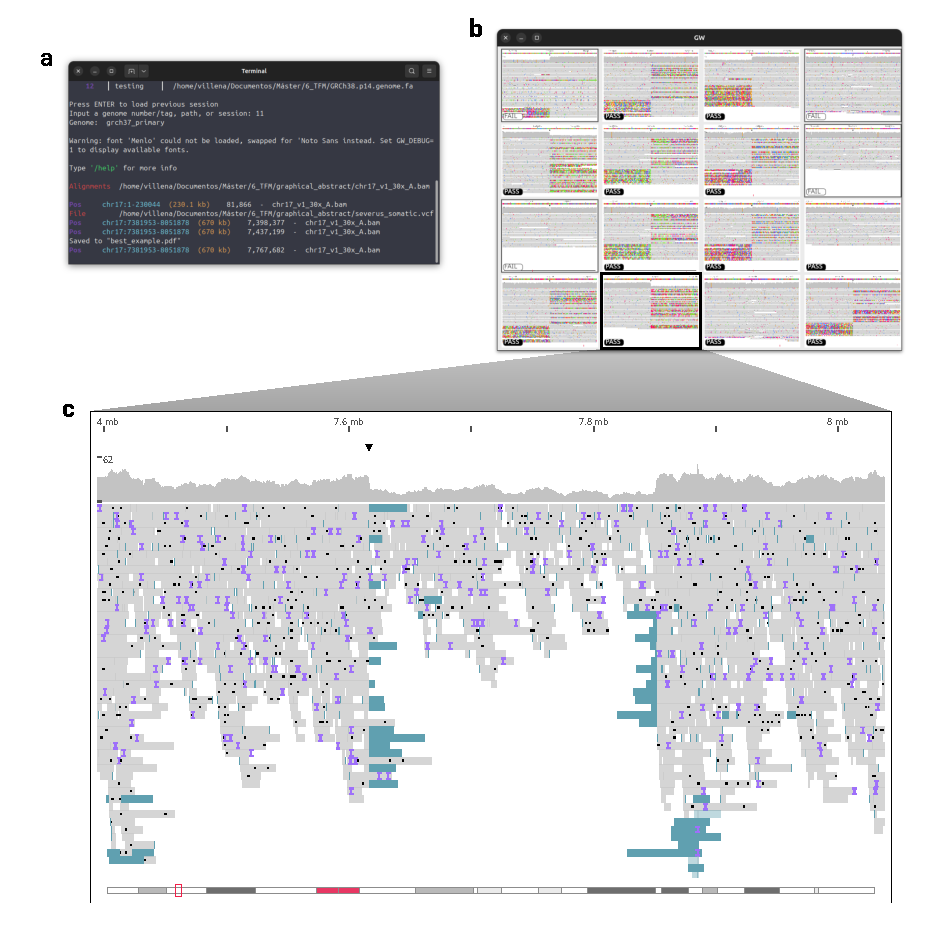
\includegraphics[width=\textwidth]{img/GW_UI.pdf}
    \caption[Alignment-based SV Validation using GW]{Alignment-based SV 
    Validation using GW. The tool is launched through the terminal, initially 
    prompting for reference genome selection (\textbf{a}) and opening an empty graphical
    window. Loading BAM and SV-containing VCF files by dragging them into the 
    graphical window generates a grid of thumbnail images corresponding to 
    VCF-indicated breakpoints (\textbf{b}). Hovering over an image displays breakpoint 
    coordinates in the terminal, while clicking opens a detailed alignment view 
    with chromosome-wide navigation capabilities (\textbf{c}). Users can return to the 
    image grid and toggle True/False buttons in the lower-left corners to track 
    SV validation status, which can be exported as a list for further analysis.}
    \label{fig:GW_UI}
\end{figure}

\end{document}